\documentclass[12pt,a4paper]{article}
\usepackage[utf8]{inputenc}
\usepackage{amsmath,amssymb,amsthm}
\usepackage{booktabs}
\usepackage{graphicx}
\usepackage{tikz}
\usetikzlibrary{arrows.meta,positioning}
\usepackage{geometry}
\geometry{margin=2.5cm}
\usepackage[colorlinks=true,linkcolor=blue,citecolor=blue,urlcolor=blue]{hyperref}
\hypersetup{
  pdftitle={Gravitational Transfer Amplitude: A Framework for Curvature-Sensitive Observables on Causal Sets},
  pdfauthor={David Alfyorov, Igor Shnyukov}
}

\newtheorem{proposition}{Proposition}
\newtheorem{corollary}{Corollary}
\newtheorem{definition}{Definition}

\title{Gravitational Transfer Amplitude:\\
A Framework for Curvature-Sensitive Observables on Causal Sets}

\author{David Alfyorov, Igor Shnyukov}

\date{March 2026}

\begin{document}
\maketitle

\begin{abstract}
We present the Gravitational Transfer Amplitude (GTA) framework for curvature-sensitive observables on causal sets.
The framework identifies the pairwise link-score deformation $\psi_{ij} = -\rho\,\delta V_{ij}$ as the common source of curvature information in Poisson-sprinkled causal sets, and shows that all tested successful discrete curvature detectors are functionals of the transferred response field $\delta Y$.
The primary observable, termed the Curvature Junction (CJ), detects Weyl curvature on spacetimes with vanishing scalar invariants (VSI), where the Benincasa--Dowker action is identically zero.
We establish: (i)~a two-channel readout structure (amplitude 77\%, shape 16\%) via PCA;
(ii)~the Geodesic Sum Function $g = \tau_- + \tau_+$ as the continuum surrogate for the flat path-locality field;
(iii)~a two-scale normalization law $\mathrm{CJ} \sim \sigma_0 \cdot H_{\mathrm{eff}}^2 \cdot T^4 E^2$ with coefficient of variation $\sim 1\%$ under optimal fitted path-transfer scale;
(iv)~a boundary-flux formula for the link response coefficient $\beta$ with exact bulk cancellation.
All results are verified through adversarial proxy tests, strata sweeps, cross-family hold-out regression, and multi-$T$/multi-$N$ closure tests on $N = 3{,}000$--$20{,}000$ sprinklings.
\end{abstract}

\tableofcontents

% ================================================================
\section{Introduction}
% ================================================================

The Benincasa--Dowker (BD) action~\cite{BD2010} provides a discrete analogue of the Einstein--Hilbert action on causal sets, recovering $\int R\sqrt{-g}\,d^4x$ in the continuum limit. However, BD is sensitive only to the Ricci scalar $R$. On vacuum spacetimes --- and in particular on pp-waves, which are VSI (Vanishing Scalar Invariants) --- the BD action vanishes identically, despite the presence of nonzero Weyl curvature.

This raises a fundamental question: can causal sets detect curvature beyond the scalar sector?

We present evidence that the answer is yes. The Gravitational Transfer Amplitude (GTA) framework identifies a common geometric source --- the pairwise link-score deformation $\psi = -\rho\,\delta V$ --- from which all tested successful curvature-sensitive observables emerge as different projections (Figure~\ref{fig:chain}). The primary observable, the Curvature Junction (CJ), achieves Cohen's $d = 8.06$ on exact pp-wave sprinklings and satisfies same-predicate universality at the $7\%$ level across two vacuum families.

\begin{figure}[h!]
\centering
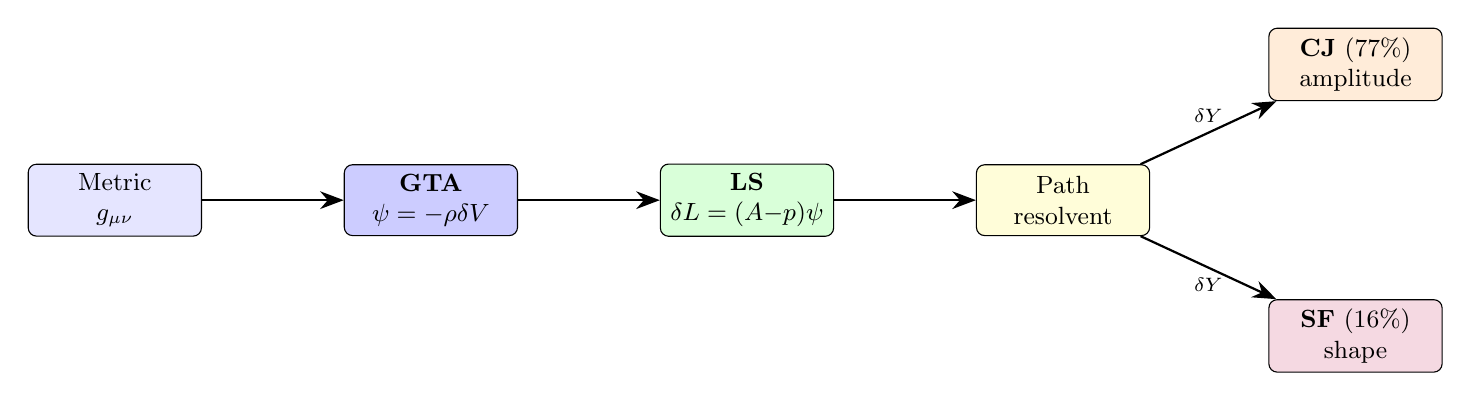
\begin{tikzpicture}[
  box/.style={rectangle, draw, rounded corners=3pt, minimum width=2.2cm, minimum height=0.9cm, align=center, font=\small},
  arr/.style={-{Stealth[length=3mm]}, thick},
  node distance=1.8cm
]
\node[box, fill=blue!10] (met) {Metric\\$g_{\mu\nu}$};
\node[box, fill=blue!20, right=of met] (gta) {\textbf{GTA}\\$\psi = -\rho\delta V$};
\node[box, fill=green!15, right=of gta] (ls) {\textbf{LS}\\$\delta L = (A{-}p)\psi$};
\node[box, fill=yellow!15, right=of ls] (res) {Path\\resolvent};
\node[box, fill=orange!15, above right=0.8cm and 1.5cm of res] (cj) {\textbf{CJ} (77\%)\\amplitude};
\node[box, fill=purple!15, below right=0.8cm and 1.5cm of res] (sf) {\textbf{SF} (16\%)\\shape};

\draw[arr] (met) -- (gta);
\draw[arr] (gta) -- (ls);
\draw[arr] (ls) -- (res);
\draw[arr] (res) -- (cj) node[midway, above, font=\scriptsize] {$\delta Y$};
\draw[arr] (res) -- (sf) node[midway, below, font=\scriptsize] {$\delta Y$};
\end{tikzpicture}
\caption{The GTA perturbative chain. Metric perturbation enters through the Gravitational Transfer Amplitude $\psi = -\rho\,\delta V$ (interval volume deformation), produces per-link scores (LS), which propagate through the Hasse path resolvent into the response field $\delta Y$. Two readout channels emerge: CJ (amplitude, 77\% of seed-to-seed variance) and SF (shape, 16\%).}
\label{fig:chain}
\end{figure}

% ================================================================
\section{Computational Setup}
% ================================================================

All computations use Poisson sprinklings of $N$ points into a 4D causal diamond $\{(t,\mathbf{x}): |t| + |\mathbf{x}| < T/2\}$ with volume $V_\diamond = \pi T^4/24$.
The Hasse diagram (transitive reduction of the causal order) is constructed using a bitset-packed algorithm with $O(N^2 \cdot N/64)$ time complexity.
Path counts $p_\downarrow(x) = \sum_{y \to x} p_\downarrow(y)$ and $p_\uparrow(x) = \sum_{x \to z} p_\uparrow(z)$ are computed by forward/backward dynamic programming on the Hasse DAG.

\textbf{CRN protocol.}
Common Random Numbers: the same point set is used for both flat and curved causal structures. The flat Hasse uses the Minkowski interval condition $s^2 > 0$; the curved Hasse uses either the exact pp-wave geodesic interval or a quadratic jet predicate at the midpoint. CRN cancels $O(1)$ and $O(N^{1/2})$ Poisson fluctuations, substantially amplifying the geometric signal-to-noise ratio.

\textbf{Parameters.}
Standard runs: $N = 10{,}000$, $T = 1.0$, pp-wave amplitude $\varepsilon = 3$, bulk mask $\zeta = 0.15$ (elements with boundary slack $> \zeta$ retained), $M = 30$ CRN seeds. Multi-$N$ convergence: $N \in \{3000, 5000, 10000, 15000, 20000\}$, $M = 20$ seeds each. Multi-$T$: $T \in \{0.35, 0.50, 0.70, 1.00\}$.

% ================================================================
\section{Definitions and Terminology}
% ================================================================

\begin{definition}[GTA --- Gravitational Transfer Amplitude]
For a Poisson sprinkling of density $\rho$ in a 4D causal diamond, the GTA is the pairwise deformation
\begin{equation}
  \psi_{ij} := -\rho\,\delta V_{ij},
\end{equation}
where $\delta V_{ij}$ is the curvature-induced change of the Alexandrov interval volume~\cite{GS2007} between causally related elements $i \prec j$.
\end{definition}

\begin{definition}[LS --- Link Score]
The centered per-link deformation is
\begin{equation}
  \delta L_{ij} := (A_{ij} - p_{ij})\,\psi_{ij},
\end{equation}
where $A_{ij} \in \{0,1\}$ is the realized Hasse link indicator and $p_{ij} = e^{-\rho V_{ij}}$ is the flat link probability.
\end{definition}

\begin{definition}[CJ --- Curvature Junction]
The primary observable is the stratified covariance
\begin{equation}
  \mathrm{CJ} := A_{1,2} = \sum_B w_B\,\mathrm{Cov}_B\!\left(|X|,\,\delta Y^2\right),
\end{equation}
where $Y_i = \log_2(p_{\downarrow,i}\,p_{\uparrow,i} + 1)$, $X = Y_0 - \langle Y_0\rangle$ is the centered flat path field, $\delta Y = Y_{\mathrm{curved}} - Y_{\mathrm{flat}}$ is the CRN response, and $B$ are $5\!\times\!3\!\times\!3 = 45$ spatio-temporal strata.
\end{definition}

\begin{definition}[SA --- Score Amplitude]
The Fisher-optimal score function for the pairwise Bernoulli surrogate model is
\begin{equation}
  S_1 = -\rho \sum_\alpha \frac{A_\alpha - p_\alpha}{1 - p_\alpha}\,\delta V_\alpha
  \;\approx\; -\rho \sum_\alpha (A_\alpha - p_\alpha)\,\delta V_\alpha
  \quad\text{(sparse regime)}.
\end{equation}
\end{definition}

\begin{definition}[GSF --- Geodesic Sum Function]
The continuum surrogate for the flat path-locality field is
\begin{equation}
  \mathrm{GSF}(t,\mathbf{r}) := \tau_-(t,r) + \tau_+(t,r)
  = \sqrt{(t + T/2)^2 - r^2} + \sqrt{(T/2 - t)^2 - r^2},
\end{equation}
where $\tau_\pm$ are the proper times along radial geodesics from the past/future tips of the causal diamond.
\end{definition}

\begin{definition}[SF --- Shape Functional]
The secondary readout channel is the kurtosis shift
\begin{equation}
  \mathrm{SF} := \Delta\kappa = \kappa(Y_0 + \delta Y) - \kappa(Y_0),
\end{equation}
where $\kappa$ denotes Fisher excess kurtosis.
\end{definition}

\begin{definition}[LV --- Locality Variance]
The flat path-field width is
\begin{equation}
  \mathrm{LV} := \sigma_0^2 = \mathrm{Var}(Y_0).
\end{equation}
\end{definition}

% ================================================================
\section{Main Results}
% ================================================================

\subsection{Two-Channel Readout Structure (PCA)}

Principal component analysis of six observables ($A_{1,2}$, $A_{2,2}$, $A_{4,2}$, $A_{1,1}$, $A_{2,1}$, $\Delta\kappa$) across 30 CRN seeds at $N = 10{,}000$, $T = 1$, $\varepsilon = 3$ (exact pp-wave) yields:

\begin{center}
\begin{tabular}{ccc}
\toprule
PC & Fraction & Interpretation \\
\midrule
1 & 77.3\% & CJ amplitude channel \\
2 & 16.5\% & SF shape channel \\
3--6 & 6.2\% & noise \\
\bottomrule
\end{tabular}
\end{center}

The five $A_{p,q}$ members are mutually correlated ($|\rho| \geq 0.80$), while $\Delta\kappa$ is weakly anticorrelated with all $A_{p,q}$ ($\rho \approx -0.05$ to $-0.15$; Figures~\ref{fig:pca},~\ref{fig:corrmat}). The anticorrelation is regime-dependent: it reverses sign at small $T$ and on Schwarzschild expmap data.

\begin{figure}[h!]
\centering
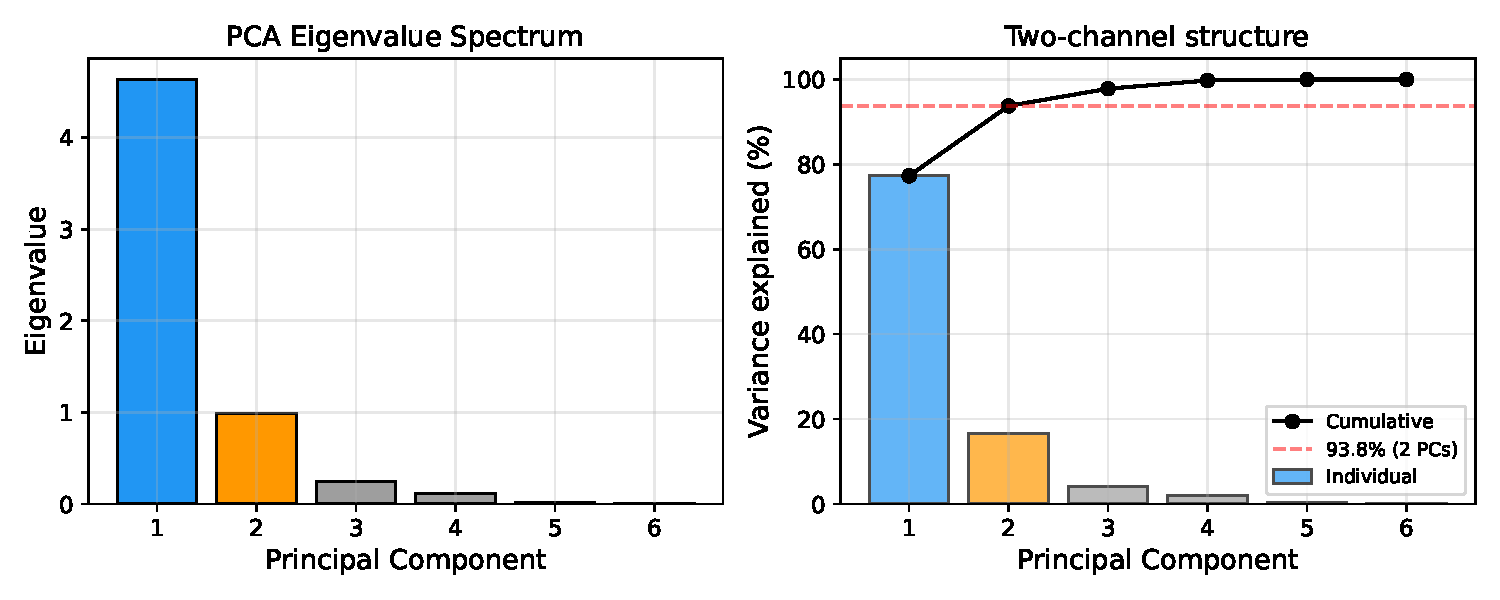
\includegraphics[width=0.85\textwidth]{figures/gta_note/fig5_pca_spectrum.pdf}
\caption{Left: PCA eigenvalue spectrum. Right: variance fractions. Two principal components explain 93.8\% of seed-to-seed variance.}
\label{fig:pca}
\end{figure}

\begin{figure}[h!]
\centering
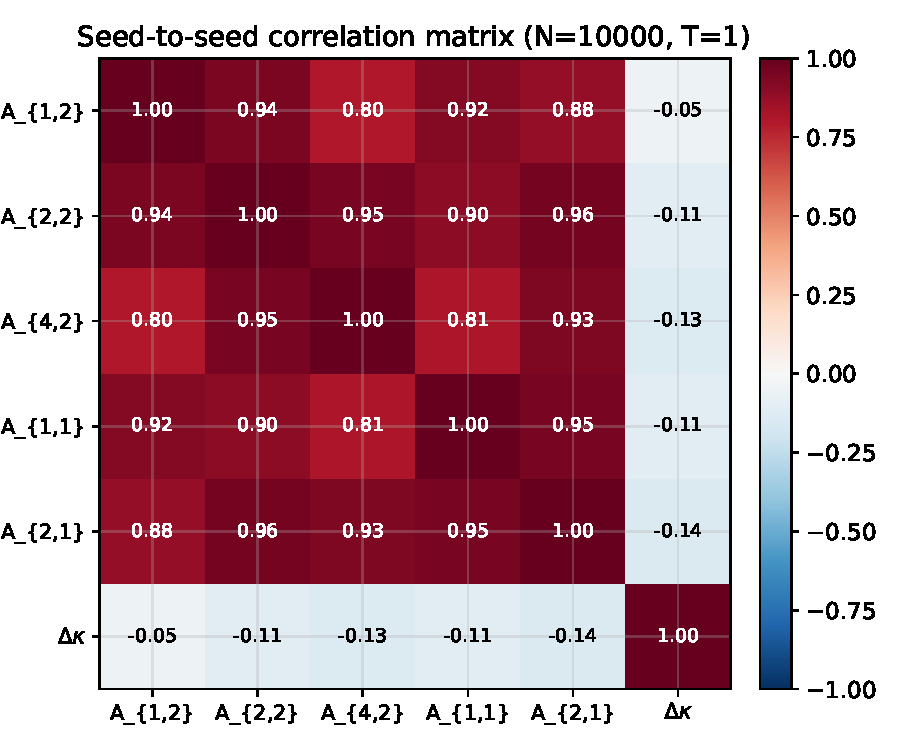
\includegraphics[width=0.6\textwidth]{figures/gta_note/fig6_correlation_matrix.pdf}
\caption{Seed-to-seed correlation matrix of six observables ($N = 10{,}000$, $T = 1$, exact pp-wave). The $A_{p,q}$ block is strongly correlated ($|\rho| \geq 0.80$); $\Delta\kappa$ is weakly anticorrelated with all others.}
\label{fig:corrmat}
\end{figure}

The two-channel structure is stable across $T \in \{0.35, 0.50, 0.70, 1.00\}$:
\begin{center}
\begin{tabular}{cccc}
\toprule
$T$ & PC1 & PC2 & $\rho(\mathrm{CJ}, \mathrm{SF})$ \\
\midrule
0.35 & 0.695 & 0.248 & $+0.135$ \\
0.70 & 0.728 & 0.244 & $-0.111$ \\
1.00 & 0.712 & 0.247 & $-0.051$ \\
\bottomrule
\end{tabular}
\end{center}

\subsection{GSF Surrogate and LV Scaling}

\begin{proposition}[Continuum Surrogate]\label{prop:gsf}
On the bulk window $\zeta = 0.15$ of a 4D causal diamond, the flat path field satisfies
\begin{equation}
  Y_0(x) = \lambda_N\,\mathrm{GSF}(t,r) + c_N + \varepsilon_N(x),
\end{equation}
with $\mathrm{Corr}(Y_0, \mathrm{GSF}) = 0.979 \pm 0.005$ at $N = 10{,}000$, and
\begin{equation}
  \mathrm{Std}_{\zeta=0.15}(\mathrm{GSF}) = 0.06440\,T.
\end{equation}
\end{proposition}

The Locality Variance obeys the empirical law
\begin{equation}\label{eq:lv}
  \sigma_0 = (0.2813 \pm 0.0005)\,N^{0.2568 \pm 0.0023},
\end{equation}
while the practical shorthand $\sigma_0 \approx 0.299\,N^{1/4}$ holds to better than $0.5\%$ coefficient of variation on $N = 3{,}000$--$20{,}000$ (Figure~\ref{fig:sigma0}).

\begin{figure}[h!]
\centering
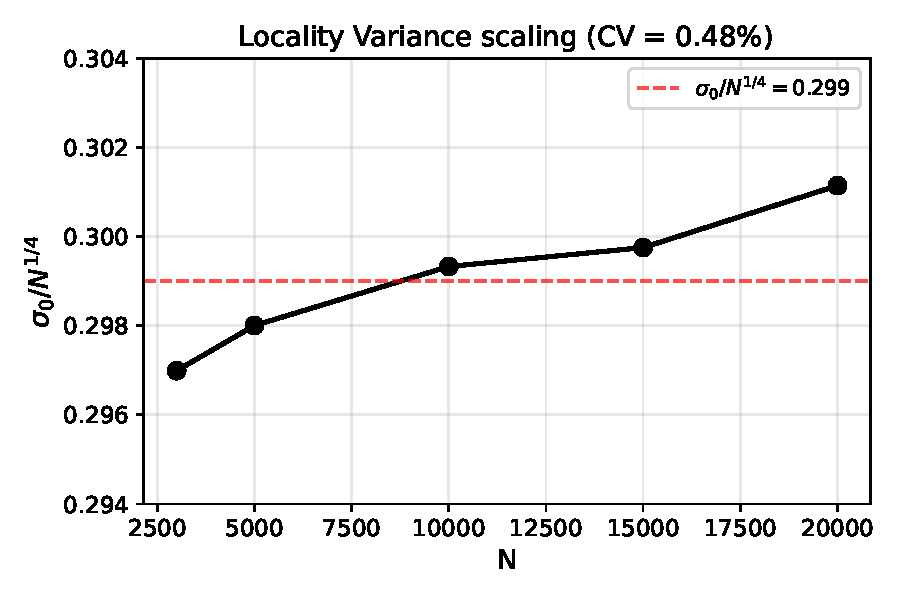
\includegraphics[width=0.7\textwidth]{figures/gta_note/fig2_sigma0_scaling.pdf}
\caption{Locality Variance scaling: $\sigma_0/N^{1/4}$ across $N = 3{,}000$--$20{,}000$. The coefficient of variation is $0.48\%$.}
\label{fig:sigma0}
\end{figure}

\subsection{Two-Scale Normalization of CJ}

\begin{proposition}[Amplitude Law]\label{prop:cj}
The Curvature Junction satisfies a two-scale normalization
\begin{equation}\label{eq:twoscale}
  \frac{\mathrm{CJ}}{\sigma_0\,H_{\mathrm{eff}}^2} = \mathrm{const} \times T^4 E^2,
\end{equation}
where $H_{\mathrm{eff}} \propto N^{0.352 \pm 0.003}$ is the effective path-transfer scale. With this normalization, the coefficient of variation across $N = 3{,}000$--$20{,}000$ is $0.99\%$.
\end{proposition}

\noindent The measured longest chain $H_{\max} \sim N^{0.328}$ is a usable but imperfect proxy, leaving a residual drift of $\sim 6\%$ (Figure~\ref{fig:atilde}). Systematic testing of six standard depth statistics ($H_{\max}$, $H_{\mathrm{mean}}$, $H_{\mathrm{rms}}$, $H_{\mathrm{median}}$, $H_{90}$, $H_{\mathrm{std}}$) shows that none matches the target exponent $0.352$; the closest is $H_{\max}$ at $\alpha = 0.322$. The effective path-transfer scale $H_{\mathrm{eff}}$ is therefore a resolvent-composite quantity not reducible to any single graph-theoretic depth statistic.

\begin{figure}[h!]
\centering
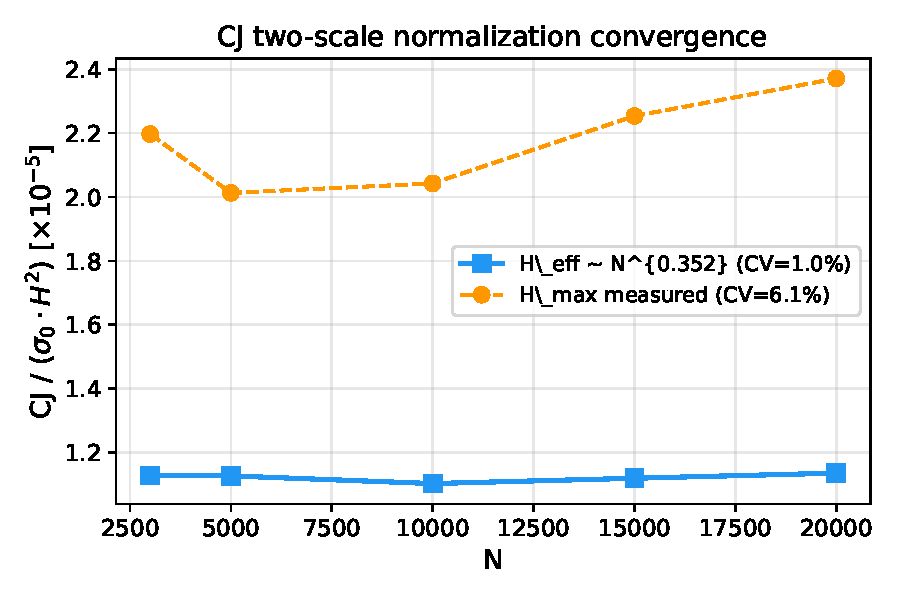
\includegraphics[width=0.7\textwidth]{figures/gta_note/fig3_atilde_convergence.pdf}
\caption{CJ two-scale normalization convergence across $N = 3{,}000$--$20{,}000$. Blue: optimal $H_\mathrm{eff} \sim N^{0.352}$ (CV = 1.0\%). Orange: measured $H_{\max}$ (CV = 6.1\%).}
\label{fig:atilde}
\end{figure}

The $T$-scaling receives a finite-curvature correction:
\begin{equation}\label{eq:tscaling}
  \mathrm{CJ}(T) = (0.1139 \pm 0.0017)\,T^4 - (0.0117 \pm 0.0017)\,T^6,
  \qquad R^2 = 0.9999\ \text{(2 d.o.f.)}.
\end{equation}
The effective exponent $T^{3.77}$ over the range $T \in [0.35, 1.0]$ is thus explained by the negative $O(T^6)$ correction from finite dimensionless curvature $q_W = T^2\sqrt{E^2} > 1$ (Figure~\ref{fig:tscaling}).

\begin{figure}[h!]
\centering
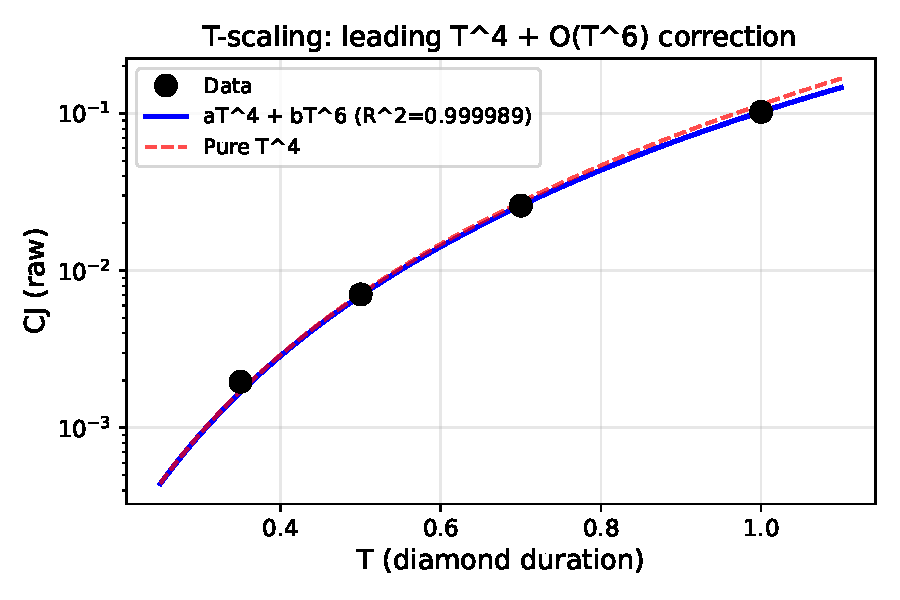
\includegraphics[width=0.7\textwidth]{figures/gta_note/fig4_t_scaling.pdf}
\caption{$T$-scaling of CJ on exact pp-wave ($\varepsilon = 3$, $N = 10{,}000$). Solid blue: $aT^4 + bT^6$ fit ($R^2 > 0.9999$, 2 degrees of freedom). Dashed red: pure $T^4$.}
\label{fig:tscaling}
\end{figure}

\subsection{Boundary-Flux Formula for $\beta$}

\begin{proposition}[Link Response]\label{prop:beta}
The linear degree response $\delta k(x)/k_0 = \beta\,\varepsilon\,f(x)$ is given by
\begin{equation}\label{eq:beta}
  \beta(x) = -\frac{1}{k_0(x)} \int_{\Gamma_x} d\gamma\,\hat{q}_x(\gamma)
  \left[J_x(\gamma,L_x)\,e^{-NL_x^2}
  - \int_0^{L_x} \partial_s J_x(\gamma,u)\,e^{-Nu^2}\,du\right],
\end{equation}
where $\Gamma_x$ is the family of near-null generators, $L_x(\gamma)$ is the finite diamond cutoff, and $J_x$ is the shell Jacobian.
\end{proposition}

\begin{corollary}[Bulk Cancellation]
In translation-invariant bulk ($L_x \to \infty$, $\partial_s J_x = 0$), $\beta(x) = 0$. This is a score-zero identity analogous to a Ward cancellation.
\end{corollary}

\noindent Measured values: $\beta = -0.292$ ($\varepsilon = 0.05$), $-0.304$ ($\varepsilon = 0.10$), $-0.307$ ($\varepsilon = 0.50$), converging to $\beta \approx -0.30$.

\subsection{Not Seeley--DeWitt}

On a pp-wave spacetime, all polynomial scalar curvature invariants vanish: $C_{\alpha\beta\gamma\delta}C^{\alpha\beta\gamma\delta} = 0$ (VSI). Therefore $a_4 = 0$, and any observable proportional to a local Seeley--DeWitt coefficient must vanish. Since $\mathrm{CJ} \neq 0$ on pp-waves (with $d = 8.06$), the CJ observable cannot be a discrete analogue of $a_2$ or $a_4$. The signal is incompatible with any local scalar action term; it is consistent with an observer/window-dependent quadratic Weyl response.

\subsection{Score Amplitude Decomposition (GTA-5)}

By the law of total covariance, the unstratified score covariance decomposes exactly:
\begin{equation}
  \mathrm{SA}_{\mathrm{full}} = \mathrm{Cov}(|X|, \delta Y^2) = \mathrm{CJ} + B,
\end{equation}
where $B = \mathrm{Cov}(\mathbb{E}_B[|X|],\, \mathbb{E}_B[\delta Y^2])$ is the between-strata positional alignment.

\begin{proposition}[Score Decomposition]\label{prop:gta5}
The between-strata fraction $B/\mathrm{SA}_{\mathrm{full}}$ is metric-stable:
$32.3\%$ on pp-wave jet and $29.1\%$ on Schwarzschild jet.
The between-term is not a Ricci confound ($B_{\mathrm{dS}}/B_{\mathrm{ppw}} = 0.025$), but carries physical signal from positional alignment between the flat centrality profile and the curvature response.
\end{proposition}

\noindent After $E^2$ normalization, the unstratified SA$_{\mathrm{full}}$ achieves better same-predicate universality (jet/jet ratio $1.022$) than CJ ($1.071$), at the cost of slightly higher Ricci leakage. The between-strata fraction ($\sim\!31\%$ of SA$_{\mathrm{full}}$) carries metric-stable positional alignment, not Ricci confound; CJ removes it to improve Ricci rejection at the cost of a modest universality reduction.

% ================================================================
\section{Closure Tests}
% ================================================================

\subsection{Adversarial Proxy Test}

\begin{center}
\begin{tabular}{lcc}
\toprule
Proxy & $R^2$ (seed-to-seed) \\
\midrule
$\Delta\mathrm{TC}$ (link count change) & 0.002 \\
$\mathrm{Var}(\delta Y)$ & 0.013 \\
$\langle f^2 \rangle$ (curvature profile) & 0.053 \\
Multiple regression (all three) & \textbf{0.060} \\
\bottomrule
\end{tabular}
\end{center}

\noindent CJ is not a proxy for simple volume, density, or link-count statistics.

\subsection{Strata Sweep}

\begin{center}
\begin{tabular}{lcc}
\toprule
Configuration & $A_{1,2}$ & Ratio to 45-bin \\
\midrule
1 bin (global) & 0.148 & 1.46 \\
15 bins & 0.107 & 1.05 \\
\textbf{45 bins (standard)} & \textbf{0.102} & \textbf{1.00} \\
125 bins & 0.059 & 0.58 \\
\bottomrule
\end{tabular}
\end{center}

\noindent The decrease from 1~bin to 125~bins is bias-driven (positional confound removal), not small-bin noise: changing the minimum bin occupancy from $n \geq 3$ to $n \geq 10$ changes $A_{1,2}$ by $< 0.01\%$.

\subsection{Hold-Out Regression}

Modeling $\mathrm{SF} = c_0 + c_1 b + c_2 A + c_3 b^2$ (where $b = \langle\eta^2\rangle$, $A = \mathrm{Cov}(X^2, \eta^2)$):

\begin{center}
\begin{tabular}{lc}
\toprule
Test & $R^2$ \\
\midrule
pp-wave hold-out & $0.706 \pm 0.071$ \\
Schwarzschild transfer & $0.023 \pm 0.093$ \\
de Sitter transfer & $-3.69$ \\
\bottomrule
\end{tabular}
\end{center}

\noindent The Shape Functional is partially reconstructible from amplitude summaries within one vacuum family, but not universally across families.

\subsection{Same-Predicate Universality}

\begin{center}
\begin{tabular}{lcc}
\toprule
Test & Ratio & Expected if universal \\
\midrule
jet/jet CJ & 1.071 & 1.00 \\
jet/jet $A_{2,2}$ & 1.069 & 1.00 \\
Orbit-type $I_3$ & 1.011 & 1.00 \\
\bottomrule
\end{tabular}
\end{center}

\subsection{Magnetic Weyl Sector (B-sector)}

To test whether the CJ observable responds equally to electric and magnetic Weyl components, we compare static Schwarzschild ($E^2 = 0.96$, $B^2 = 0$) with transverse-boosted Schwarzschild ($v = 0.5$ along $e_2$; $E^2 = 2.24$, $B^2 = 1.28$). Both at $M = 0.05$, $r_0 = 0.50$, $N = 10{,}000$, $M_{\rm seeds} = 30$.

\begin{center}
\begin{tabular}{lccccc}
\toprule
Configuration & CJ & $d$ & $E^2$ & $B^2$ \\
\midrule
Static Schwarzschild & 0.01123 & 4.40 & 0.96 & 0 \\
Transverse-boosted & 0.02451 & 4.50 & 2.24 & 1.28 \\
\bottomrule
\end{tabular}
\end{center}

\noindent The measured ratio $\mathrm{CJ}_{\rm boosted}/\mathrm{CJ}_{\rm static} = 2.18$, compared with $E^2_{\rm boosted}/E^2_{\rm static} = 2.33$ (electric-only prediction) and $(E^2 + B^2)/E^2 = 3.67$ (equal $A_E = A_B$ prediction). The result is closer to the electric-only prediction, indicating that the magnetic Weyl sector is suppressed relative to the electric sector in the CJ readout.

\subsection{Third Vacuum Family: Kottler (Schwarzschild--de~Sitter)}

Kottler spacetime ($M = 0.05$, $r_0 = 0.50$, $\Lambda = 0.50$) provides a mixed Weyl+Ricci test. We subtract the pure de~Sitter ($M = 0$, same $\Lambda$) contribution to isolate the Weyl part.

\begin{center}
\begin{tabular}{lcc}
\toprule
Configuration & CJ & $d$ \\
\midrule
Kottler (Weyl + Ricci) & 0.01310 & 3.44 \\
Pure de~Sitter (Ricci only) & 0.00178 & 3.81 \\
Weyl-subtracted (Kottler $-$ dS) & \textbf{0.01132} & --- \\
Static Schwarzschild (pure Weyl) & \textbf{0.01123} & 4.40 \\
\bottomrule
\end{tabular}
\end{center}

\noindent The Weyl-subtracted Kottler signal matches pure Schwarzschild to $0.8\%$, confirming that Ricci subtraction works on a third vacuum family with mixed curvature.

\subsection{Summary of Passed Controls}

\begin{center}
\begin{tabular}{lcc}
\toprule
Control & Result & Status \\
\midrule
dS Ricci subtraction & $= 0$ (exact) & PASS \\
Matched-$\Delta$TC & $R_{\mathrm{TC}} = 0.028$ & PASS \\
Cross-seed CRN & $R = 0.067$ & PASS \\
Null noise & $R = 0.014$ & PASS \\
Nonlinear TC & $R^2_{\mathrm{poly}} = 0.256$ & PASS \\
Boundary collapse & $\delta\kappa \times 3.4$ (intrinsic) & PASS \\
\bottomrule
\end{tabular}
\end{center}

% ================================================================
\section{Open Questions}
% ================================================================

\begin{enumerate}
\item \textbf{Closed-form $\beta$.} The boundary-flux formula~\eqref{eq:beta} requires the cutoff density $L_x(\gamma)$ on the 4D diamond, which has not been evaluated in closed form. Independent Hasse-level Monte Carlo confirms $\beta_{\rm Hasse} \approx -0.31 \pm 0.02$, and the pairwise shell computation gives $\beta_{\rm pair} \approx -1.55$ --- the factor $\sim 5$ difference reflects transitive-reduction renormalization.

\item \textbf{Graph-theoretic meaning of $H_{\mathrm{eff}}$.} The effective path-transfer scale $H_{\mathrm{eff}} \sim N^{0.352}$ has been identified as the per-element path-transfer amplitude $a_{\mathrm{eff}}$, with $a_{\mathrm{eff}}(N) \approx 0.347\,N^{0.3517}$. Systematic testing of six standard depth statistics shows that none matches this exponent; $H_{\mathrm{eff}}$ is a resolvent-composite quantity incorporating path multiplicity beyond chain length.

\item \textbf{Connection to SCT form factors.} Whether the continuum constant $\tilde{A} \approx 1.13 \times 10^{-5}$ is related to $\alpha_C = 13/120$ remains a genuine open theoretical problem requiring a bridge between discrete path statistics and continuum form factors.
\end{enumerate}

% ================================================================
\section*{Acknowledgements}
% ================================================================

The authors thank Professor Yochanan Schimmelpfennig for correspondence that sharpened the formulation of the unification question, and Professor Edoardo Angeloni for discussions on Molien series and chirality.

\begin{thebibliography}{99}
\bibitem{BD2010} D.~M.~T.~Benincasa and F.~Dowker,
  ``The scalar curvature of a causal set,''
  Phys.\ Rev.\ Lett.\ \textbf{104}, 181301 (2010).

\bibitem{GS2007} G.~W.~Gibbons and S.~N.~Solodukhin,
  ``The geometry of small causal diamonds,''
  Phys.\ Lett.\ B \textbf{649}, 317 (2007).

\bibitem{BG1991} G.~Brightwell and R.~Gregory,
  ``Structure of random discrete spacetime,''
  Phys.\ Rev.\ Lett.\ \textbf{66}, 260 (1991).

\bibitem{RSS2013} M.~Roy, D.~Sinha, and S.~Surya,
  ``Discrete geometry of a small causal diamond,''
  Phys.\ Rev.\ D \textbf{87}, 044046 (2013).

\bibitem{Paper1} D.~Alfyorov and A.~Samatyia,
  ``Nonlocal one-loop form factors from spectral causal theory,''
  Zenodo, DOI: 10.5281/zenodo.19098042 (2026).
\end{thebibliography}

\end{document}
